\documentclass[xcolor=table,dvipsnames]{beamer}
  \definecolor{lg}{rgb}{.85,.85,.85}
  \usepackage{graphicx}


  \usecolortheme[named=teal]{structure}
  \setbeamerfont{frametitle}{size = {\large}, family=\sffamily}
  \setbeamertemplate{navigation symbols}{}
  % packages for extra math symbols
  \usepackage{amsthm, amsmath, amssymb} 

  % I like these fonts better
  \usepackage{mathpazo}

  \usepackage{tikz}
  \usetikzlibrary{arrows}
  \usetikzlibrary{decorations.markings}
  \tikzstyle{dot}=[circle, inner sep=.4mm, draw=black, outer sep=2mm, fill=black]
  \tikzstyle{gdot}=[circle, inner sep=.4mm, draw=black!25, outer sep=2mm,
                    fill=black!25]
  \tikzstyle{odot}=[circle, inner sep=.4mm, draw=black, outer sep=2mm]

  \usepackage{pgfplots}
  \pgfplotsset{compat=1.8}

  \DeclareMathOperator{\Av}{Av}

  \newcommand{\Avn}{\Av_n(123)}
  \newcommand{\Avns}{\Av_n^*(123)}

  \newcommand{\num}{\nu}
  \newcommand{\ds}{\displaystyle}
  \newcommand{\ra}{\rightarrow}
  \newcommand{\R}{\mathbb{R}}
  \newcommand{\sg}{\sigma}
  \renewcommand{\S}{\mathfrak{S}}
  \newcommand{\C}{\mathcal{C}}

  \newcommand{\Ex}[1]{\mathbb{E}\left[ #1 \right]}

% ===================================================================== %
\begin{document}


\title[Patterns in Permutations]%
  {\Large Counting Patterns: \\ \large Equipopularity in Permutation Classes}

\author{Cheyne Homberger \\[1pc] \small
University of Maryland, Baltimore County \\ 
US Department of Defense }

\date{\small Howard University \\ 2016}


\begin{frame}
  \titlepage
\end{frame}

% \begin{frame} 
%   \begin{center}
%     \rmfamily \LARGE \color{teal}{Introduction}
%   \end{center}
% \end{frame}

\begin{frame} \frametitle{Plotting Permutations}
  \begin{block}{Definition}
    If $\pi$ is a permutation of length $n$, then the \emph{plot}
    of $\pi$ is the set of points 
    $$ \{ (1, \pi(1)), (2, \pi(2)), \cdots (n, \pi(n)) \} \subset \mathbb{R}^2 $$
  \end{block}

  \pause 
  \begin{center}
  \begin{tikzpicture}[scale = .5,
                      dot/.style={circle, fill=teal, inner sep=.5mm}]
    \draw[<->] (0,6) -- (0,0) -- (6,0);
    \foreach \y [count = \x] in {3,5,1,4,2}{
    % \node[dot, label=210:{{\tiny $(\x,\y)$}}] at (\x,\y) {};
      \node[dot] at (\x,\y) {};
      \draw (\x,-.25) -- (\x, .25);
      \draw (-.25, \x) -- (.25, \x);
    }
    \pause
    {\scriptsize
    \node[anchor=south west] at (1,3) {3};
    \pause
    \node[anchor=south west] at (2,5) {5};
    \pause
    \node[anchor=south west] at (3,1) {1};
    \pause
    \node[anchor=south west] at (4,4) {4};
    \pause
    \node[anchor=south west] at (5,2) {2};
    }
  \end{tikzpicture}
  \end{center}
  \uncover<2->{
  $$ \pi = 35142 $$
  }
\end{frame}

\begin{frame} \frametitle{Dots on a Plane} 
  \only<1->{
  \begin{block}{Definition} 
    Let $A$ and $B$ be two sets of $n$ points in $\R^2$, each with the property
    that no two points lie on the same horizontal or vertical line. \\
    Say that $A$ is \emph{order isomorphic} to $B$ (denoted $A \sim B$) if $A$
    can be transformed into $B$ by stretching, contracting, and translating the
    axes horizontally and vertically.
  \end{block}
  }
  
  \vspace{.5pc}

  \pause 

  \begin{block}{Example}
    \vspace{1pc}
    \begin{tikzpicture}[scale = .45,
                        dot/.style={circle, fill=teal, inner sep=.5mm}]
      \node[dot] at (1,3.5) {};
      \node[dot] at (1.3,4.5) {};
      \node[dot] at (3,.5) {};
      \node[dot] at (3.4,4) {};
      \node[dot] at (5,1) {};
      {\scriptsize
      \uncover<5->{\node[anchor=south west] at (3,.5) {1};}
      \uncover<6->{\node[anchor=south west] at (5,1) {2};}
      \uncover<7->{\node[anchor=south west] at (1,3.5) {3};}
      \uncover<8->{\node[anchor=south west] at (3.4,4) {4};}
      \uncover<9->{\node[anchor=south west] at (1.3,4.5) {5};}
      }
    \end{tikzpicture}
    \hspace{1pc}
    \raisebox{2.5pc}{$\sim$}
    \hspace{1pc}
    \begin{tikzpicture}[scale = .45,
                        dot/.style={circle, fill=teal, inner sep=.5mm}]
      \node[dot] at (1,2) {};
      \node[dot] at (2.5,5) {};
      \node[dot] at (3,1) {};
      \node[dot] at (3.5,4) {};
      \node[dot] at (5,1.5) {};
      {\scriptsize
      \uncover<5->{\node[anchor=south west] at (3,1) {1};}
      \uncover<6->{\node[anchor=south west] at (5,1.5) {2};}
      \uncover<7->{\node[anchor=south west] at (1,2) {3};}
      \uncover<8->{\node[anchor=south west] at (3.5,4) {4};}
      \uncover<9->{\node[anchor=south west] at (2.5,5) {5};}
      }
    \end{tikzpicture}
    \hspace{1pc}
    \pause
    \raisebox{2.5pc}{$\sim$}
    \hspace{1pc}
    \begin{tikzpicture}[scale = .45,
                        dot/.style={circle, fill=teal, inner sep=.5mm}]
      \foreach \y [count = \x] in {3,5,1,4,2}
      \node[dot] at (\x,\y) {};
      {\scriptsize
      \uncover<5->{\node[anchor=south west] at (3,1) {1};}
      \uncover<6->{\node[anchor=south west] at (5,2) {2};}
      \uncover<7->{\node[anchor=south west] at (1,3) {3};}
      \uncover<8->{\node[anchor=south west] at (4,4) {4};}
      \uncover<9->{\node[anchor=south west] at (2,5) {5};}
      }
    \end{tikzpicture}

    \pause
    \vspace{1pc}
    { \hfill $\pi = 35142$ \hspace{2pc}}
  \end{block}
\end{frame}

% ====================================================================== %


\begin{frame}{Pattern Occurrences}
  \uncover<1->{
  \begin{block}{Patterns}
    Say that one permutation $\pi$ contains another permutation $\sg$ \emph{as
    a pattern} (denoted $\sg \prec \pi$) if the plot of $\pi$ contains a subset
    which is equivalent to the plot of $\sg$. The number of occurrences of
    $\sg$ in $\pi$ (denoted $\nu_\sg(\pi)$) is the number of such subsets.
  \end{block}
  }
  \uncover<2->{
  \begin{center}
  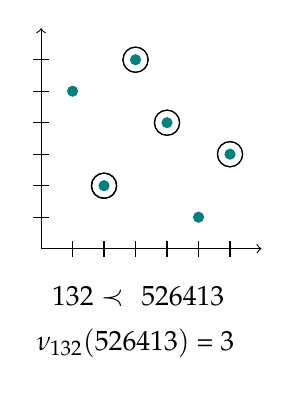
\begin{tikzpicture}[scale = .4,
                      dot/.style={circle, fill=teal, inner sep=.5mm}]
    \draw[->] (0,0) -- (7,0);
    \draw[->] (0,0) -- (0,7);
    \foreach \y [count = \x] in {5,2,6,4,1,3}{
      \node[dot] at (\x,\y) {};
      \draw (\x, -.25) -- (\x,.25);
      \draw (-.25, \x) -- (.25, \x);
    }

    \uncover<4>{
      \draw (2,2) circle (4mm);
      \draw (3,6) circle (4mm);
      \draw (6,3) circle (4mm);
    }

    \uncover<5>{
      \draw (2,2) circle (4mm);
      \draw (3,6) circle (4mm);
      \draw (4,4) circle (4mm);
    }

    \uncover<6>{
      \draw (2,2) circle (4mm);
      \draw (4,4) circle (4mm);
      \draw (6,3) circle (4mm);
    }

    \node at (4.5,-1.5) {$ 526413 $};
    \node at (1.5, -1.5) {$ 132 \prec $};

    \uncover<3->{
      \node at (3, -3) {$\nu_{132}(526413)$ = 3};
    }
  \end{tikzpicture}
  \end{center}
  }
\end{frame}

\begin{frame}{Random Data}
  \begin{center}
    % \begin{tikzpicture}[scale=4, only marks]
    % \draw (-0.05,-0.05) -- (1.05,-0.05) -- (1.05,1.05) -- (-0.05,1.05) -- cycle;
    % \draw plot[mark=*, mark size = .1mm] file {organizeddata.txt};
    % \end{tikzpicture}
    \only<1-3>{\input{without_regline.pgf}}\only<4>{\input{with_regline.pgf}}
  \end{center}

  \vspace{-1pc}
  
  \pause
  $$
  \rowcolors{1}{teal!0}{teal!10}
  \begin{array}{cc|c}
    \num_{12} &\num_{21} & \text{Avg}\\
    2803 & 2147 & 2475
  \end{array}
  $$
  \pause
  $$
  \rowcolors{1}{teal!0}{teal!10}
  \begin{array}{cccccc|c}
    \num_{123} &\num_{132} &\num_{213} &\num_{231} 
      &\num_{312} &\num_{321} & \text{Avg}\\
    35357 & 30063 & 31414 & 22321 & 23348 & 19197 & 26950
  \end{array}
  $$
\end{frame}

\begin{frame}{Random Restricted Data}
  \begin{center}
    % \begin{tikzpicture}[scale=4, only marks]
    % \draw (-0.05,-0.05) -- (1.05,-0.05) -- (1.05,1.05) -- (-0.05,1.05) -- cycle;
    % \draw plot[mark=*, mark size = .1mm] file {organizeddata.txt};
    % \end{tikzpicture}
    \only<1-3>{\input{avoid_without_regline.pgf}}\only<4>{\input{avoid_with_regline.pgf}}
  \end{center}

  \vspace{-1pc}
  
  \pause
  $$
  \rowcolors{1}{teal!0}{teal!10}
  \begin{array}{cc|c}
    \num_{12} &\num_{21} & \text{Avg}\\
    685 & 4265 & 2475
  \end{array}
  $$
  \pause
  $$
  \rowcolors{1}{teal!0}{teal!10}
  \begin{array}{cccccc|c}
    \num_{123} &\num_{132} &\num_{213} &\num_{231} 
      &\num_{312} &\num_{321} & \text{Avg}\\
    2426 & 0 & 14874 & 15208 & 14896 & 114296 & 26950
  \end{array}
  $$
\end{frame}



\begin{frame}{Patterns as Random Variables}
  \begin{block}{Theorem (B\'ona 2007)}
    For a (uniformly) randomly selected permutation of length $n$, 
    the random variables $\num_{\sg}$ are asymptotically normal as $n$
    approaches infinity.
  \end{block}

  \pause

  \begin{block}{Theorem (Janson, Nakamura, Zeilberger 2013)}
    For a randomly selected permutation of length $n$ and two patterns $\sg$
    and $\rho$, the random variables $\num_{\sg}$ and $\num_{\rho}$ are
    asymptotically jointly normally distributed as $n \rightarrow \infty$. 
  \end{block}
\end{frame}


\begin{frame}{Motivation}
  \begin{block}{Fact}
    In $\S_n$, the number of occurrences of a specific pattern depends only on
    the length of the pattern. That is, for a pattern $\sg \in \S_k$, we have 
    $$ \num_{\sg} (\S_n) = \frac{n!}{k!} \binom{n}{k}.$$
  \end{block}

  \pause
  \begin{block}{Question}
  How does this change when we replace $\S_n$ with a 
  proper permutation class?
  \end{block}
  \pause

  \begin{figure}
  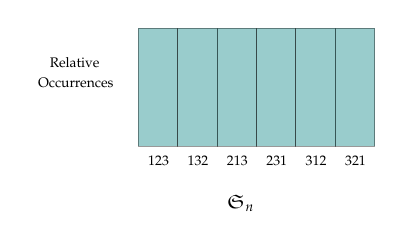
\begin{tikzpicture}
  [scale = .5]
  \foreach \x in {0,1,2,3,4,5}{
    \draw[color = black, fill = teal, opacity = .4] (\x,0) rectangle (\x+1, 3);
  }
  \draw (0, 0) node[anchor=north west] {\tiny $123$};
  \draw (1, 0) node[anchor=north west] {\tiny $132$};
  \draw (2, 0) node[anchor=north west] {\tiny $213$};
  \draw (3, 0) node[anchor=north west] {\tiny $231$};
  \draw (4, 0) node[anchor=north west] {\tiny $312$};
  \draw (5, 0) node[anchor=north west] {\tiny $321$};
  \draw (2,-1) node[anchor=north west] {\scriptsize $\S_n$};
  \draw (-2.5, 2.5) node[anchor=north west] {\tiny Relative};
  \draw (-2.8, 2) node[anchor=north west] {\tiny Occurrences};
  \end{tikzpicture} \hspace{2pc} \pause
  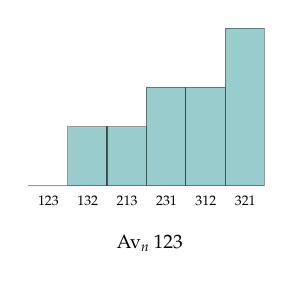
\begin{tikzpicture}
  [scale = .5]
  \foreach \x/\y in {0/0, 1/1.5, 2/1.5, 3/2.5, 4/2.5, 5/4}{
    \draw[color = black, fill = teal, opacity = .4] (\x,0) rectangle (\x+1,\y );
  }
  \draw (0, 0) node[anchor=north west] {\tiny $123$};
  \draw (1, 0) node[anchor=north west] {\tiny $132$};
  \draw (2, 0) node[anchor=north west] {\tiny $213$};
  \draw (3, 0) node[anchor=north west] {\tiny $231$};
  \draw (4, 0) node[anchor=north west] {\tiny $312$};
  \draw (5, 0) node[anchor=north west] {\tiny $321$};
  \draw (2,-1) node[anchor=north west] {\scriptsize $\Av_n 123$};
  \end{tikzpicture}
  \end{figure}
\end{frame}

\begin{frame}{Equipopularity}
  \begin{block}{Definition}
    The \emph{popularity} of a pattern $\sigma$ in a class $C$ is equal to 
    $$ \sum_{n\geq 1} \num_\sigma (C_n). $$
  \end{block}

  \begin{block}{Definition}
    Patterns are said to be \emph{equipopular} if they have the same number 
    of occurrences (within a specified set or across two different sets). 
  \end{block}
\end{frame}

\begin{frame}{Equipopularity --- Example}
  \begin{block}{Fact}
    For a class $C$ and a pattern $\sigma$, we have 
    $$ \num_\sigma(C_n) = 
      |\{ (\pi; \sigma) : \pi \in C_n,\ \sigma \prec \pi\}|.$$
  \end{block}
  \pause

  \begin{block}{Proposition}
    In the class $\Av(132)$, $\sigma$ and $\sigma^{-1}$ are equipopular.
  \end{block}
  \begin{proof}
    This follows from the fact that $\pi$ avoids $132$ if and only if $\pi^{-1}$ 
    avoids $132$, and the fact that $\sigma \prec \pi$ if and only if 
    $\sigma^{-1} \prec \pi^{-1}$. 
  \end{proof}
\end{frame}


% ====================================================================== %


\begin{frame}{Motivation}
  \pause
  \begin{block}{Theorem (B\'ona 2010)}
    Within the class $\Av(132)$:
    $$\num_{213} = \num_{231} = \num_{312}.$$
  \end{block}
  \pause
  \begin{block}{Theorem (Rudolph 2013)}
    If two patterns \emph{have the same structure}, then they
    are equipopular within $\Av(132)$. 
  \end{block}
  \pause
  \begin{block}{Theorem (Chua, Sankar 2013)}
    If two patterns are equipopular in $\Av(132)$, then they \emph{have the same
    structure}. 
  \end{block}
  % \pause
  % \begin{block}{Corollary}
  %   The equipopularity classes within $\Av(132)$ are in bijection with the
  %   set of integer partitions. 
  % \end{block}
\end{frame}


\begin{frame}{Separable Permutations}
  \pause
  \begin{block}{Definition}
    The \emph{separable permutations} are those which avoid both $2413$ and
    $3142$. We denote the class $\Av(2413,3142)$ by $S$. 
  \end{block}
  \pause
  \begin{block}{Theorem (Albert, H, Pantone)}
    Two patterns are equipopular in the separables if and only if they
    \emph{have the same structure}. Further, the equipopularity classes are in 
    bijection with the set of integer partitions.
  \end{block}
\end{frame}


\begin{frame}{Separable Permutations}
  \begin{block}{Definition}
    Given two permutations $\pi$ and $\sigma$, their \emph{direct sum} ($\pi
    \oplus \sigma$) and \emph{skew sum} ($\pi \ominus \sigma$) are defined as
    follows:
  \end{block}
  \begin{center}
    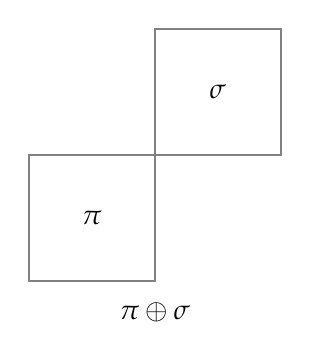
\begin{tikzpicture}[scale=.8]
      \draw[thick,draw=black!50] (0,0) rectangle (2,2);
      \draw[thick,draw=black!50] (2,2) rectangle (4,4);
      \node at (1,1) {$\pi$};
      \node at (3,3) {$\sigma$};
      \node at (2,-.5) {$\pi \oplus \sigma$};
    \end{tikzpicture}
    \hspace{2pc}
    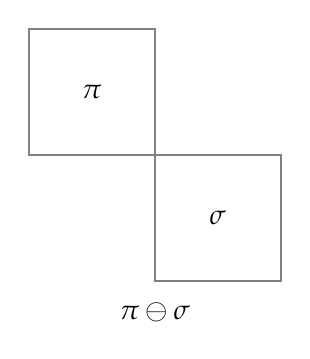
\begin{tikzpicture}[scale=.8]
      \draw[thick,draw=black!50] (0,2) rectangle (2,4);
      \draw[thick,draw=black!50] (2,0) rectangle (4,2);
      \node at (1,3) {$\pi$};
      \node at (3,1) {$\sigma$};
      \node at (2,-.5) {$\pi \ominus \sigma$};
    \end{tikzpicture}
  \end{center}
\end{frame}


\begin{frame}{Separable Permutations}
  \begin{block}{Alternate Definition}
    The separable permutations are those which can be constructed via arbitrary
    skew and direct sums of the permutation $1$. 
  \end{block}
  \pause
  \begin{block}{Example}
    The permutation $\pi = 215643798$ is separable, since 
    $$ \pi = \Big(1 \ominus 1\Big) \oplus \Big( (1 \oplus 1) \ominus 
       1 \ominus 1 \Big) \oplus 1 \oplus \Big(1 \ominus 1\Big).$$
  \end{block}
\end{frame}

\begin{frame}{Separable Permutations}
  $$ \pi = 215643798 = 
      \Big(1 \ominus 1\Big) \oplus \Big( (1 \oplus 1) \ominus 
     1 \ominus 1 \Big) \oplus 1 \oplus \Big(1 \ominus 1\Big).$$
  \begin{center}
  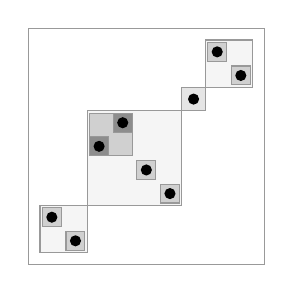
\begin{tikzpicture}[scale=.3]

    \uncover<3-5,8->{
      \draw[draw=black!40, fill opacity=.4, fill=black!10] 
        (.5,.5) rectangle (2.5,2.5);
      \draw[draw=black!40, fill opacity=.4, fill=black!10] 
        (2.5,2.5) rectangle (6.5,6.5);
      \draw[draw=black!40, fill opacity=.4, fill=black!10] 
        (6.5,6.5) rectangle (7.5,7.5);
      \draw[draw=black!40, fill opacity=.4, fill=black!10] 
        (7.5,7.5) rectangle (9.5,9.5);
    }
    \uncover<4-5,9->{
      \draw[draw=black!40, fill opacity=.4, fill=black!40] 
        (2.6, 4.6) rectangle (4.4, 6.4);
      %\draw[draw=black!40] (4.6, 4.4) rectangle (5.4, 3.6);
      %\draw[draw=black!40] (5.6, 3.4) rectangle (6.4, 2.6);
    }

    \uncover<5,10->{
      \foreach [count=\x] \y in {2,1,5,6,4,3,7,9,8}
      \draw[draw=black!40, fill opacity=.4, fill=black!40] 
        (\x-.4,\y-.4) rectangle (\x+.4,\y+.4) {};
      \draw[draw=black!40, fill opacity=.4, fill=black!70] 
        (2.6,4.6) rectangle (3.4,5.4) {};
      \draw[draw=black!40, fill opacity=.4, fill=black!70] 
        (3.6,5.6) rectangle (4.4,6.4) {};
      \draw[draw=black!40, fill opacity=1, fill=black!10] 
        (6.5,6.5) rectangle (7.5,7.5) {};

    }
    \uncover<2->{
      \foreach [count=\x] \y in {2,1,5,6,4,3,7,9,8}{
      \node[circle,inner sep=.5mm, fill=black] at (\x,\y) {};
      }
      \draw[draw=black!40] (0,0) rectangle (10,10);
    }

  \end{tikzpicture}
  \hspace{2pc}
  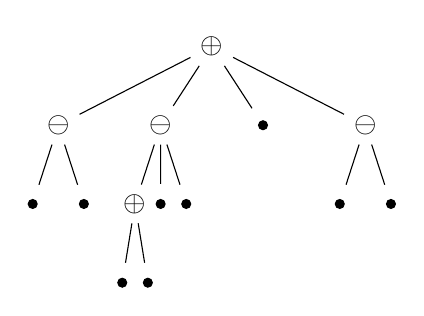
\begin{tikzpicture}[xscale=.65]
    \uncover<7->{
      \node[] (a1) at (6,5) {$\oplus$};
    }

    \uncover<8->{
      \node[] (b1) at (3,4) {$\ominus$};
      \node[] (b2) at (5,4) {$\ominus$};
      \node[] (b4) at (9,4) {$\ominus$};
      \node[dot] (b3) at (7,4) {};
      \draw (a1) -- (b1);
      \draw (a1) -- (b2);
      \draw (a1) -- (b4);
      \draw (a1) -- (b3);
    }

    \uncover<9->{
      \node (c3) at (4.5,3) {$\oplus$};
      \draw (b2) -- (c3);
    }
    \uncover<10->{
      \node[dot] (c1) at (2.5,3) {};
      \node[dot] (c2) at (3.5,3) {};
      \node[dot] (c4) at (5,3) {};
      \node[dot] (c5) at (5.5,3) {};
      \node[dot] (c6) at (8.5,3) {};
      \node[dot] (c7) at (9.5,3) {};
      \node[dot] (d4) at (4.25,2) {};
      \node[dot] (d5) at (4.75,2) {};
      \draw (b1) -- (c1);
      \draw (b1) -- (c2);
      \draw (b2) -- (c4);
      \draw (b2) -- (c5);
      \draw (b4) -- (c6);
      \draw (b4) -- (c7);
      \draw (c3) -- (d4);
      \draw (c3) -- (d5);
    }
  \end{tikzpicture}
  \end{center}
\end{frame}

% ====================================================================== %


\begin{frame}{Tree Containment}
  \pause
  \begin{center}
    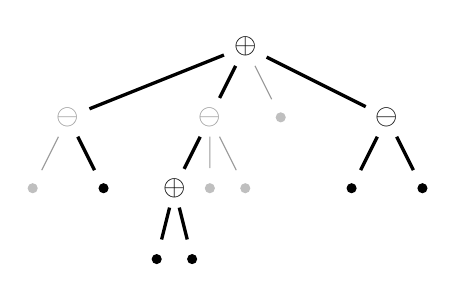
\begin{tikzpicture}[scale=.9]

      \node[] (a1) at (6,5) {$\oplus$};

      \node[] (b1) at (3.5,4) {\color{black!40}{$\ominus$}};
      \node[] (b2) at (5.5,4) {\color{black!40}{$\ominus$}};
      \node[gdot] (b3) at (6.5,4) {};
      \node[] (b4) at (8,4) {$\ominus$};

      \node[gdot] (c1) at (3,3) {};
      \node[dot] (c2) at (4,3) {};

      \node (c3) at (5,3) {$\oplus$};
      \node[gdot] (c4) at (5.5,3) {};
      \node[gdot] (c5) at (6,3) {};

      \node[dot] (c6) at (7.5,3) {};
      \node[dot] (c7) at (8.5,3) {};

      \node[dot] (d4) at (4.75,2) {};
      \node[dot] (d5) at (5.25,2) {};

      \draw[draw=black,very thick] (a1) -- (b1);
      \draw[draw=black, very thick] (a1) -- (b2);
      \draw[draw=black!40] (a1) -- (b3);
      \draw[draw=black, very thick] (a1) -- (b4);

      \draw[draw=black!40] (b1) -- (c1);
      \draw[draw=black, very thick] (b1) -- (c2);

      \draw[draw=black, very thick] (b2) -- (c3);
      \draw[draw=black!40] (b2) -- (c4);
      \draw[draw=black!40] (b2) -- (c5);

      \draw[draw=black, very thick] (b4) -- (c6);
      \draw[draw=black, very thick] (b4) -- (c7);

      \draw[draw=black, very thick] (c3) -- (d4);
      \draw[draw=black, very thick] (c3) -- (d5);
    \end{tikzpicture}
    \hspace{4pc}
    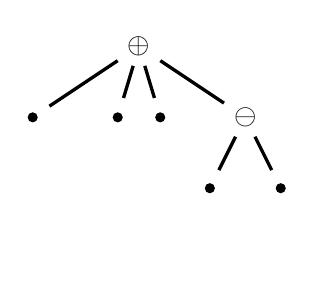
\begin{tikzpicture}[scale=.9]

      \node[] (a1) at (6,5) {$\oplus$};
      \node[dot] (b1) at (4.5,4) {};
      \node[dot] (b2) at (5.7,4) {};
      \node[dot] (b3) at (6.3,4) {};
      \node[] (b4) at (7.5,4) {$\ominus$};
      \node[dot] (c1) at (7,3) {};
      \node[dot] (c2) at (8,3) {};
      \node at (6,2) {};

      \draw[very thick] (a1) -- (b1);
      \draw[very thick] (a1) -- (b2);
      \draw[very thick] (a1) -- (b3);
      \draw[very thick] (a1) -- (b4);
      \draw[very thick] (b4) -- (c1);
      \draw[very thick] (b4) -- (c2);

    \end{tikzpicture}
  \end{center}
\end{frame}



\begin{frame}{Equipopularity}
  \begin{block}{Question}
    If two patterns are equipopular, how are their trees related?
  \end{block}
\end{frame}


\begin{frame}{Strategy}
  \pause

  \begin{block}{Part 1}
    Find the operations on trees which preserve popularity.
  \end{block}
  \pause
  \begin{block}{Part 2}
    Show that equipopularity implies that their trees are related by one of
    these operations. 
  \end{block}
\end{frame}


\begin{frame}{Preserving Popularity}
  \pause
  \begin{block}{Symmetries}
    \begin{center}
      \begin{tabular}{l|l}
      Permutation & Tree 
      \pause \\
      \hline
      Complement & Flip signs 
      \pause \\
      Reverse & Reversal and sign flip  
      \pause \\
      Inverse & Reverse children of $\ominus$ nodes
      \end{tabular}
    \end{center}
  \end{block}
  \pause
  \begin{block}{Fact}
    If two permutations (or trees) are related by any of the above 
    symmetries, then they are equipopular. 
  \end{block}
\end{frame}


\begin{frame}{Preserving Popularity - Shuffling}
  \pause
  \begin{block}{Lemma}
    Rearranging the children of any node preserves equipopularity. 
  \end{block}

  \begin{center}
    \uncover<3->{
    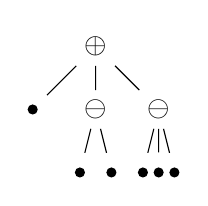
\begin{tikzpicture}[scale=.4]
    \node[label=east:{}] (A) at (5,10) {$\oplus$};
    \node[dot] (b1) at (3,8) {};
    \node (b2) at (5,8) {$\ominus$};
    \node (b3) at (7,8) {$\ominus$};
    \node[dot] (c1) at (4.5,6) {};
    \node[dot] (c2) at (5.5,6) {};
    \node[dot] (c3) at (6.5,6) {};
    \node[dot] (c4) at (7,6) {};
    \node[dot] (c5) at (7.5,6) {};
    \foreach \to/\from in 
      {A/b1, A/b2, A/b3, b2/c1, b2/c2, b3/c3, b3/c4, b3/c5}
    \draw (\to) -- (\from);
    \end{tikzpicture}
    }
    \hspace{2pc}
    \uncover<5->{
    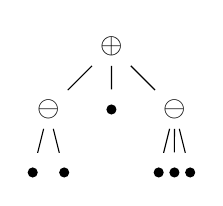
\begin{tikzpicture}[scale=.4]
    \node[label=east:{}] (A) at (5,10) {$\oplus$};
    \node[dot] (b1) at (5,8) {};
    \node (b2) at (3,8) {$\ominus$};
    \node (b3) at (7,8) {$\ominus$};
    \node[dot] (c1) at (2.5,6) {};
    \node[dot] (c2) at (3.5,6) {};
    \node[dot] (c3) at (6.5,6) {};
    \node[dot] (c4) at (7,6) {};
    \node[dot] (c5) at (7.5,6) {};
    \foreach \to/\from in 
      {A/b1, A/b2, A/b3, b2/c1, b2/c2, b3/c3, b3/c4, b3/c5}
    \draw (\to) -- (\from);
    \end{tikzpicture}
    }

    \vspace{1pc}
    \pause
    
    \uncover<4->{
    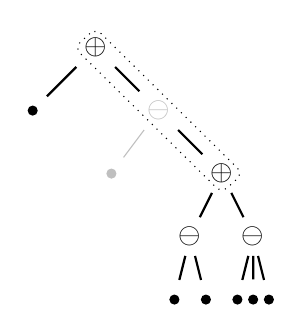
\begin{tikzpicture}[scale=.4]
    \node (A1) at (5,10) {$\oplus$};
    \node (A2) at (7,8) {\color{black!25}{$\ominus$}};
    \node (A3) at (9,6) {$\oplus$};
    \node[dot] (d1) at (3,8) {};
    \node[gdot] (d2) at (5.5,6) {};
    \node (B1) at (8,4) {$\ominus$};
    \node (B2) at (10,4) {$\ominus$};
    \node[dot] (c1) at (7.5,2) {};
    \node[dot] (c2) at (8.5,2) {};
    \node[dot] (c3) at (9.5,2) {};
    \node[dot] (c4) at (10,2) {};
    \node[dot] (c5) at (10.5,2) {};
    \foreach \to/\from in {A1/d1, A1/A2, A2/A3, A3/B1, A3/B2, 
          B1/c1, B1/c2, B2/c3, B2/c4, B2/c5}
      \draw[thick] (\to) -- (\from);
    \draw[black!25] (A2) -- (d2);
    \draw[rounded corners=1mm, dotted] (A1.north) -- (A1.west) -- (A3.south) --
    (A3.east) -- cycle;
    \end{tikzpicture}
    }
   % 
    \hspace{2pc}
    \uncover<6->{
    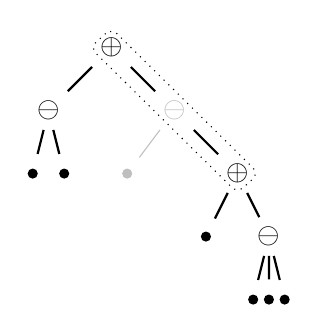
\begin{tikzpicture}[scale=.4]
    \node (A1) at (5,10) {$\oplus$};
    \node (A2) at (7,8) {\color{black!25}{$\ominus$}};
    \node (A3) at (9,6) {$\oplus$};
    \node[dot] (d1) at (8,4) {};
    \node[gdot] (d2) at (5.5,6) {};
    \node (B1) at (3,8) {$\ominus$};
    \node (B2) at (10,4) {$\ominus$};
    \node[dot] (c3) at (9.5,2) {};
    \node[dot] (c4) at (10,2) {};
    \node[dot] (c5) at (10.5,2) {};
    \node[dot] (c1) at (2.5,6) {};
    \node[dot] (c2) at (3.5,6) {};
    \foreach \to/\from in {A3/d1, A1/A2, A2/A3, A1/B1, A3/B2, 
          B1/c1, B1/c2, B2/c3, B2/c4, B2/c5}
      \draw[thick] (\to) -- (\from);
    \draw[black!25] (A2) -- (d2);
    \draw[rounded corners=1mm, dotted] (A1.north) -- (A1.west) -- (A3.south) --
    (A3.east) -- cycle;
    \end{tikzpicture}
    }
  \end{center}
\end{frame}



\begin{frame}{Preserving Popularity - Rotation}
  \pause
  \begin{block}{Lemma}
    The following operation preserves equipopularity:
  \end{block}
  \pause

  \begin{center}
    \begin{tikzpicture}[scale=.8]
      \node (top) at (2.5,5) {};
      \node[circle, draw=black, inner sep=.5mm, outer sep=2mm, 
          label=north east:{$a$}] (a) at (3,4) {};
      \node[circle, draw=black, inner sep=.5mm, outer sep=2mm, 
          label=north east:{$b$}] (b) at (4,2) {};
      \node[circle, draw=black, inner sep=.5mm, outer sep=2mm, 
          label=north east:{$c$}] (c) at (5,0) {};
      \node (bot) at (5.5,-1) {};

      \node[outer sep=4mm] (F) at (2.6,2.5) {\only<3-4>{$F$}\only<5>{$G$}};
      \node[outer sep=4mm] (G) at (3.6,0.5) {\only<3-4>{$G$}\only<5>{$F$}};

      \draw (a) -- (b);
      \draw (b) -- (c);

      \draw[dotted] (a) -- (top);
      \draw[dotted] (c) -- (bot);

      \draw[black!25] (a) -- ++(.3, -2) -- ++(-1.7,0) -- (a);
      \draw[black!25] (b) -- ++(.3, -2) -- ++(-1.7,0) -- (b);

      \only<4>{\draw[<->] (F) --  (G);}

    \end{tikzpicture}
  \end{center}
\end{frame}

\begin{frame}{Preserving Popularity}
  \begin{block}{Lemma (Albert, H, Pantone)}
    The following operations preserve popularity:
    \begin{itemize}
      \item Reversal
      \item Complementation
      \item Inversion
      \item Shuffling
      \item Rotation
    \end{itemize}
  \end{block}
\end{frame}


\begin{frame}{Canonical Representatives}
  \pause
  \begin{center}
  \begin{tikzpicture}[scale=.5]
    \node[circle, inner sep=.5mm, outer sep=1mm] (1) at (5,10) {$\oplus$};
    \node[circle, inner sep=.5mm, outer sep=1mm] (21) at (6,8) {$\ominus$};
    \node[label=below:{$\lambda_1$}] (22) at (4,8) {$\dots$};

    \node[circle, inner sep=.5mm, outer sep=1mm] (31) at (7,6) {$\oplus$};
    \node[label=below:{$\lambda_2$}] (32) at (5,6) {$\dots$};

    \node[circle, inner sep=.5mm, outer sep=1mm] (41) at (9,2) {$\circ$};
    \node[label=below:{$\lambda_{k-1}$}] (42) at (7,2) {$\dots$};

    \node[label=below:{$\lambda_{k} + 1$}] (5) at (9,0) {$\dots$};
    \node[outer sep = 3mm] (inv) at (8,4) {};

    \draw[thick, dotted] (31) -- (inv);
    \draw[thick, dotted] (41) -- (inv);
    \draw[thick, dotted] (42) -- (inv);

    \foreach \to/\from in {1/21, 1/22, 21/31, 21/32, 41/5}
      \draw (\to) -- (\from);
  \end{tikzpicture} 
    \uncover<4->{%
    \hspace{1pc}
    \raisebox{7pc}{$\equiv$}
    \hspace{1pc}
  \begin{tikzpicture}[scale=.5]
    \draw[very thick, dotted] (0,0)--(1,1) node[pos=.5, above left] {$\lambda_1$};
    \draw[very thick, dotted] (1.5,9)--(2.5,8) node[pos=.5, below left] {$\lambda_2$};
    \draw[very thick, dotted] (3,1.5)--(4,2.5) node[pos=.5, above left] {$\lambda_3$};
    \draw[very thick, dotted] (4.5,7.5)--(5.5,6.5) node[pos=.5, below left] {$\lambda_4$};
    \draw[very thick, dotted] (6,3)--(7,4) node[pos=.5, above left] {$\lambda_5$};
    \node at (8,5) {$\dots$};
    \node at (1,-1) {};
  \end{tikzpicture}
    }
  \end{center}
  \uncover<3->{%
  $$ \lambda := \lambda_1 \geq \lambda_2 \geq \dots \geq \lambda_n$$
  }
\end{frame}



\begin{frame}{The Other Direction}
  \pause

  \begin{block}{Lemma (Albert, H, Pantone)}
    If two patterns are equipopular, one can be transformed into the other by
    the above operations. 
  \end{block}

  \pause

  \begin{block}{Corollary}
    The set of equipopularity classes for patterns of length $n$ are in
    bijection with the set of partitions of the integer $n-1$. 
  \end{block}
\end{frame}


\begin{frame}{Rough Sketch of Proof}
  \pause
  \begin{block}{Idea \# 1}
    Given any arbitrary pattern, we can factor its popularity generating
    function into the popularity generating functions for monotone runs. 
  \end{block}

  \pause
  \begin{center}
  \begin{tikzpicture}[scale=.6]
    \draw[very thick, dotted] (0,0)--(1,1) node[pos=.5, above left] {$\lambda_1$};
    \draw[very thick, dotted] (1.5,9)--(2.5,8) node[pos=.5, below left] {$\lambda_2$};
    \draw[very thick, dotted] (3,1.5)--(4,2.5) node[pos=.5, above left] {$\lambda_3$};
    \draw[very thick, dotted] (4.5,7.5)--(5.5,6.5) node[pos=.5, below left] {$\lambda_4$};
    \draw[very thick, dotted] (6,3)--(7,4) node[pos=.5, above left] {$\lambda_5$};

    \node at (8,5) {$\dots$};
  \end{tikzpicture}
  \end{center}
\end{frame}



\begin{frame}{Rough Sketch of Proof}
  \pause
  \begin{block}{Idea \#2}
    Given a product of monotone popularity generating functions, we can uniquely
    factor into its component parts, and thus recover the lengths of each
    monotone pattern.
  \end{block}
  \pause
  \begin{block}{How?}
    \begin{itemize}
      \pause
      \item Recursively build a bivariate popularity generating function for all
      monotone patterns. 
      \pause
      \item Notice (or let Sage/Maple/Mathematica/Singular tell you) that these are related to the
      \emph{Gegenbauer polynomials}, a family of orthogonal polynomials. 
      \pause
      \item Use the orthogonality of these polynomials to uniquely factor any
      product.
    \end{itemize}
  \end{block}
\end{frame}


\begin{frame}{Conclusion}
  \begin{center}
  \begin{tikzpicture}[scale=.35]
    \draw[very thick, dotted] (0,0)--(1,1) node[pos=.5, above left] {$\lambda_1$};
    \draw[very thick, dotted] (1.5,9)--(2.5,8) node[pos=.5, below left] {$\lambda_2$};
    \draw[very thick, dotted] (3,1.5)--(4,2.5) node[pos=.5, above left] {$\lambda_3$};
    \draw[very thick, dotted] (4.5,7.5)--(5.5,6.5) node[pos=.5, below left] {$\lambda_4$};
    \draw[very thick, dotted] (6,3)--(7,4) node[pos=.5, above left] {$\lambda_5$};
    \node at (8,5) {$\dots$};
  \end{tikzpicture}
    \hspace{1pc}
    \raisebox{4pc}{\small $\leftrightarrow\ \lambda_1 + \lambda_2 + \dots + 
                   \lambda_{k-1} + (\lambda_k - 1)$}

    \vspace{1pc} 
    \small
    Length $n$ canonical representative $\leftrightarrow$ 
    partition of the integer $n-1$. 
  \end{center}
\end{frame}

\begin{frame} 
  \begin{center}
    \LARGE \color{teal}{Questions?}
  \end{center}
\end{frame}

\end{document}
